\documentclass[12pt, titlepage]{article}

\usepackage[a4paper, total={6in, 8in}]{geometry}

\usepackage{booktabs}
\usepackage{tabularx}
\usepackage{hyperref}
\hypersetup{
    colorlinks,
    citecolor=black,
    filecolor=black,
    linkcolor=red,
    urlcolor=blue
}
% \usepackage[round]{natbib}
\usepackage[numbers,square]{natbib}

\usepackage{graphicx}
\graphicspath{ {./images/} }

%% Comments

\usepackage{color}

\newif\ifcomments\commentstrue %displays comments
%\newif\ifcomments\commentsfalse %so that comments do not display

\ifcomments
\newcommand{\authornote}[3]{\textcolor{#1}{[#3 ---#2]}}
\newcommand{\todo}[1]{\textcolor{red}{[TODO: #1]}}
\else
\newcommand{\authornote}[3]{}
\newcommand{\todo}[1]{}
\fi

\newcommand{\wss}[1]{\authornote{blue}{SS}{#1}} 
\newcommand{\plt}[1]{\authornote{magenta}{TPLT}{#1}} %For explanation of the template
\newcommand{\an}[1]{\authornote{cyan}{Author}{#1}}

%% Common Parts

\newcommand{\progname}{ImgBeamer} % PUT YOUR PROGRAM NAME HERE
\newcommand{\authname}{Joachim de Fourestier} % AUTHOR NAMES                  

\usepackage{hyperref}
    \hypersetup{colorlinks=true, linkcolor=blue, citecolor=blue, filecolor=blue,
                urlcolor=blue, unicode=false}
    \urlstyle{same}
                                


\begin{document}

\title{Verification and Validation Report: \progname} 
\author{\authname}
\date{\today}
	
\maketitle

\pagenumbering{roman}

\section{Revision History}

\begin{tabularx}{\textwidth}{p{3cm}p{2cm}X}
\toprule {\bf Date} & {\bf Version} & {\bf Notes}\\
\midrule
2023/03/26 & 0.1.0 & Creation\\
2023/04/02 & 0.1.1 & Start requirements testing sections\\
2023/04/03 & 0.2.0 & Fill in the Functional Requirements Evaluation
  section, along with test images\\
\bottomrule
\end{tabularx}

~\newpage

\section{Symbols, Abbreviations and Acronyms}

\renewcommand{\arraystretch}{1.2}
\begin{tabular}{l l} 
  \toprule		
  \textbf{symbol} & \textbf{description}\\
  \midrule 
  GUI & Graphical User Interface\\
  SRS & Software Requirements Specification\\
  T & Test\\
  VnV & Verification and Validation\\
  \bottomrule
\end{tabular}\\

~\newline
\noindent See the SRS \cite{SRS}, VnV Plan \cite{VnV_plan}, MG \cite{MG},
and MIS \cite{MIS} Documentation for additional items.

\newpage

\tableofcontents

\listoftables %if appropriate

\listoffigures %if appropriate

\newpage

\pagenumbering{arabic}

\section{Report Purpose}
This purpose of this report is to document the tasks accomplished and
testing results as part the verification and validation process of \progname{}
as laid out in the VnV Plan \cite{VnV_plan}. The code documentation along with notes
on developer setup and testing is available at:
\url{https://joedf.github.io/ImgBeamer/jsdocs/index.html} The software design documentation
is available at: \url{https://github.com/joedf/CAS741_w23}. The source code is
available at: \url{https://github.com/joedf/ImgBeamer/tree/cas741}

\section{Functional Requirements Evaluation}
In this section, we report the measures that were taken to evaluate whether the
functional requirements (as listed in the SRS \cite{SRS}) were met.
Most of these tests were executed manually due to the complex nature of visual information, GUI testing, and
the subjectivity of image quality.

\subsection{Image Import and Export (R1 and R6)}
This section is focused on testing the image import and export functionalities.

\subsubsection{T1: Test import for PNG/JPG/BMP format (R1)}
The software could successfully load or import valid (non-corrupt) images files in the PNG, JPG, and BMP formats.
An example is shown in figure \ref{fig_t1}.
\begin{figure}[h!]
  \begin{center}
   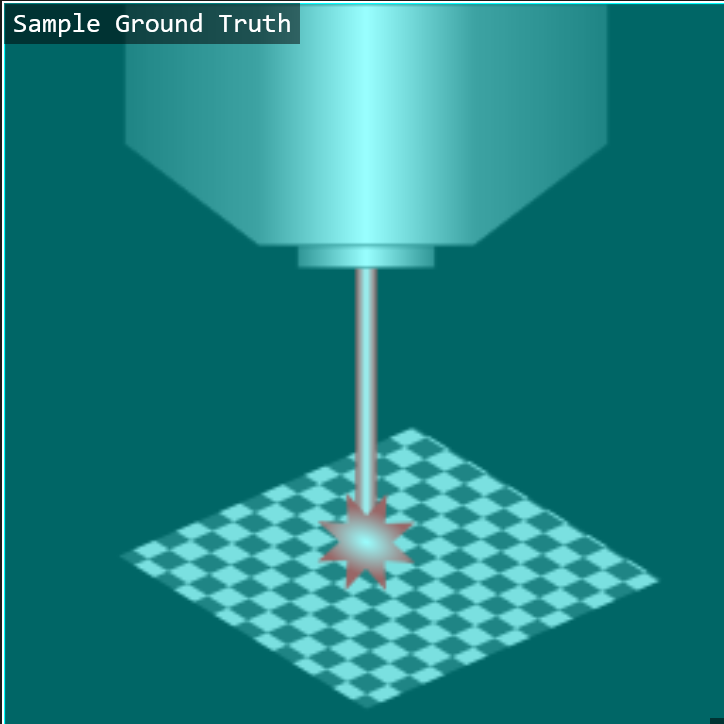
\includegraphics[width=0.5\textwidth]{t1.png}
  \caption{An example loaded test image.}
  \label{fig_t1}
  \end{center}
\end{figure}


\subsubsection{T2: Test PNG Image Export (R6)}
The software could successfully export valid PNG image files of the resulting image (see figure \ref{fig_t2}).
\begin{figure}[h!]
  \begin{center}
   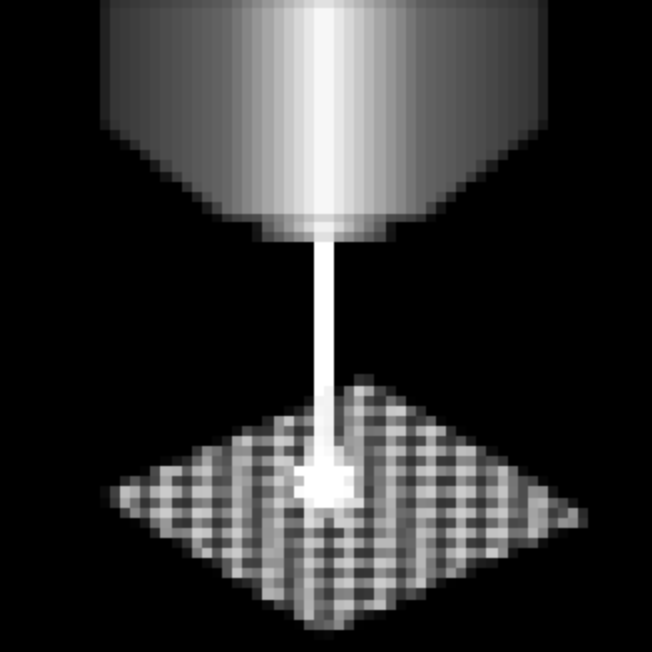
\includegraphics[width=0.5\textwidth]{t2.png}
  \caption{The image was faithfully reproduced (in grayscale with some imaging parameters change for clarity).}
  \label{fig_t2}
  \end{center}
\end{figure}

\subsection{Spot Profile and Imaging Parameters (R2, R3, R4, and R5)}
This section focuses on testing the sampling and image rendering based on the given
imaging parameters and subregion / ROI. The ground truth / input image used for these tests
is depicted in figure \ref{fig_gt0} with the cyan overlay depicting the subregion area.

\begin{figure}[h!]
  \begin{center}
   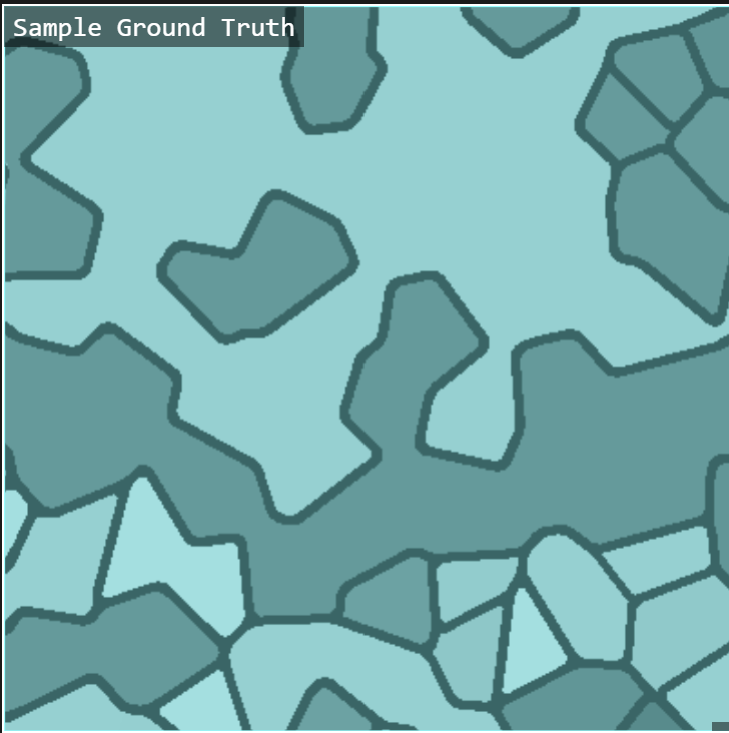
\includegraphics[width=0.5\textwidth]{gt0.png}
  \caption{The ground truth image used for testing with the subregion set to cover the entire image.}
  \label{fig_gt0} 
  \end{center}
\end{figure}


\subsubsection{T3: Spot Width and Height - Exact-sampling (R2 and R5)}
The test was passed as shown in figure \ref{fig_t3}.
\begin{figure}[h!]
  \begin{center}
   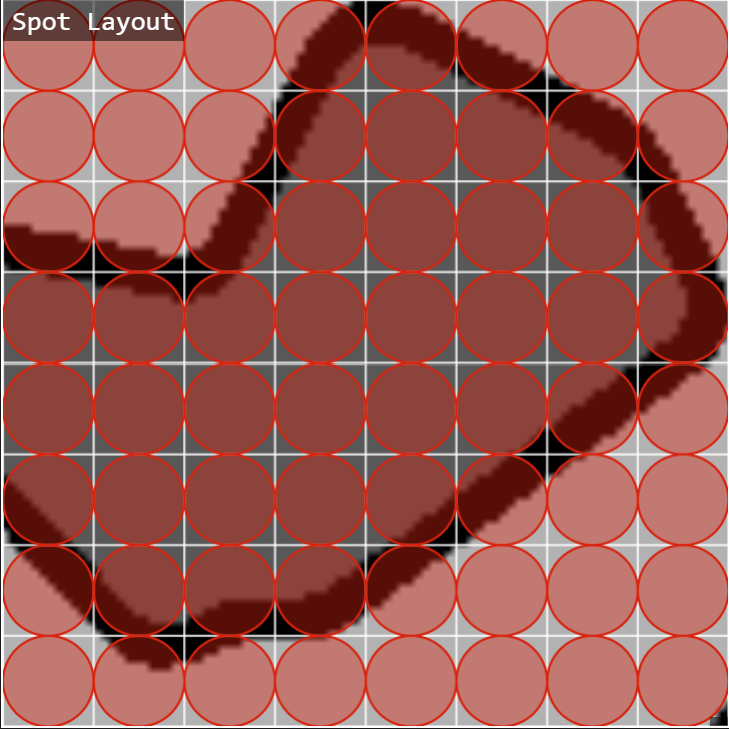
\includegraphics[width=5cm]{t3a.png}
   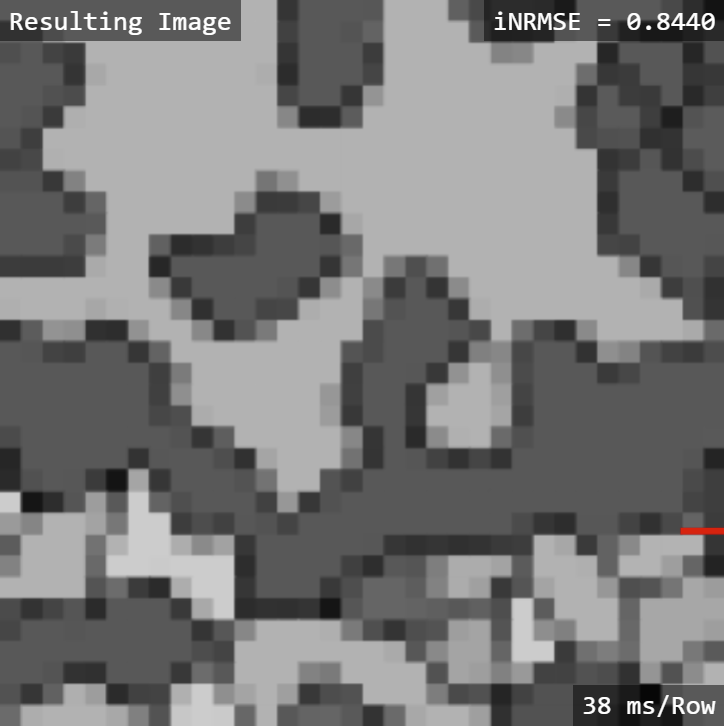
\includegraphics[width=5cm]{t3b.png}
  \caption{The spot layout and resulting image matching the expected test result:
  Spot size of 100 by 100\%.}
  \label{fig_t3} 
  \end{center}
\end{figure}

\subsubsection{T4: Spot Width and Height - Under-sampling (R2 and R5)}
The test was passed as shown in figure \ref{fig_t4}.
\begin{figure}[h!]
  \begin{center}
   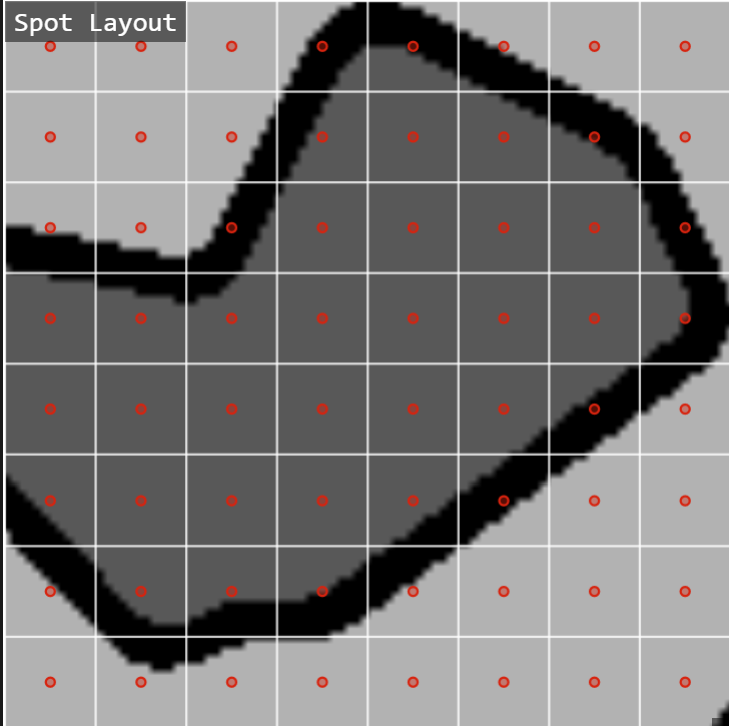
\includegraphics[width=5cm]{t4a.png}
   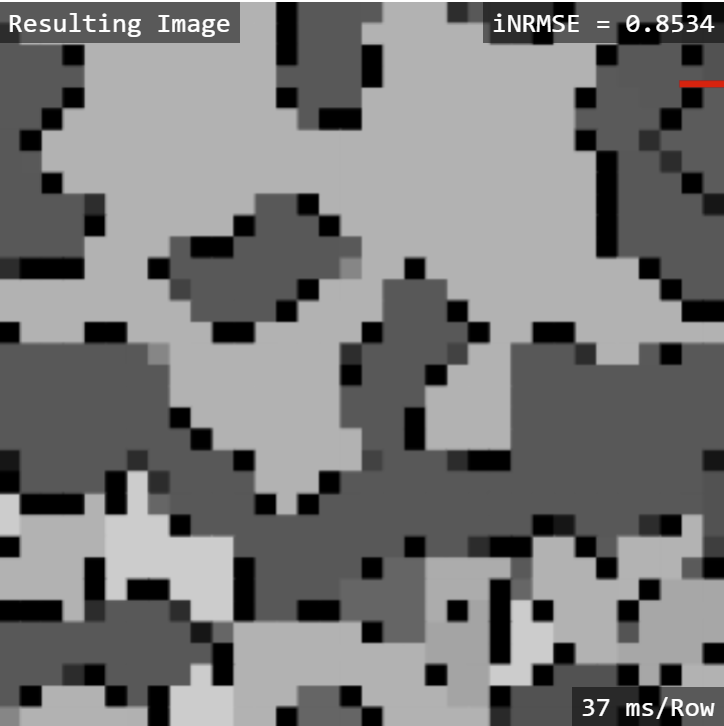
\includegraphics[width=5cm]{t4b.png}
  \caption{The spot layout and resulting image matching the expected test result:
  Spot size of 10 by 10\%.}
  \label{fig_t4} 
  \end{center}
\end{figure}

\subsubsection{T5: Spot Width and Height - Over-sampling (R2 and R5)}
The test was passed as shown in figure \ref{fig_t5}.
\begin{figure}[h!]
  \begin{center}
   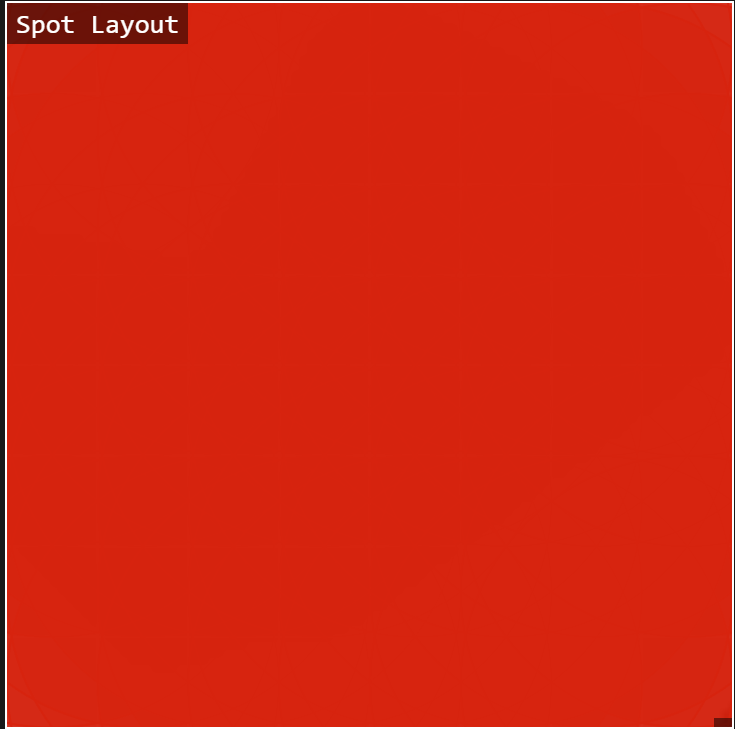
\includegraphics[width=5cm]{t5a.png}
   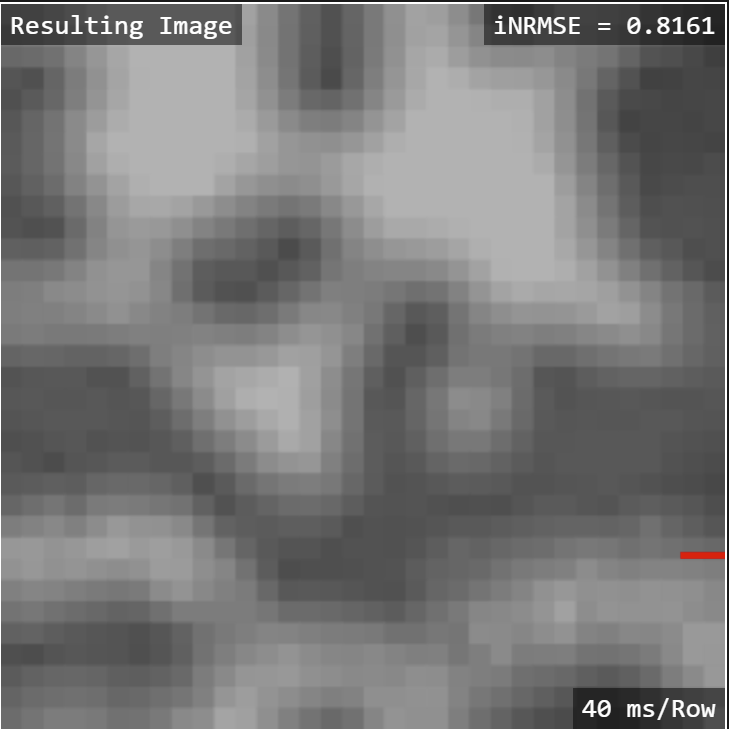
\includegraphics[width=5cm]{t5b.png}
  \caption{The spot layout and resulting image matching the expected test result:
  Spot size of 500 by 500\%.}
  \label{fig_t5} 
  \end{center}
\end{figure}

\subsubsection{T6: Spot Rotation - Astigmatism (R2 and R5)}
The test was passed as shown in figure \ref{fig_t6}.
\begin{figure}[h!]
  \begin{center}
   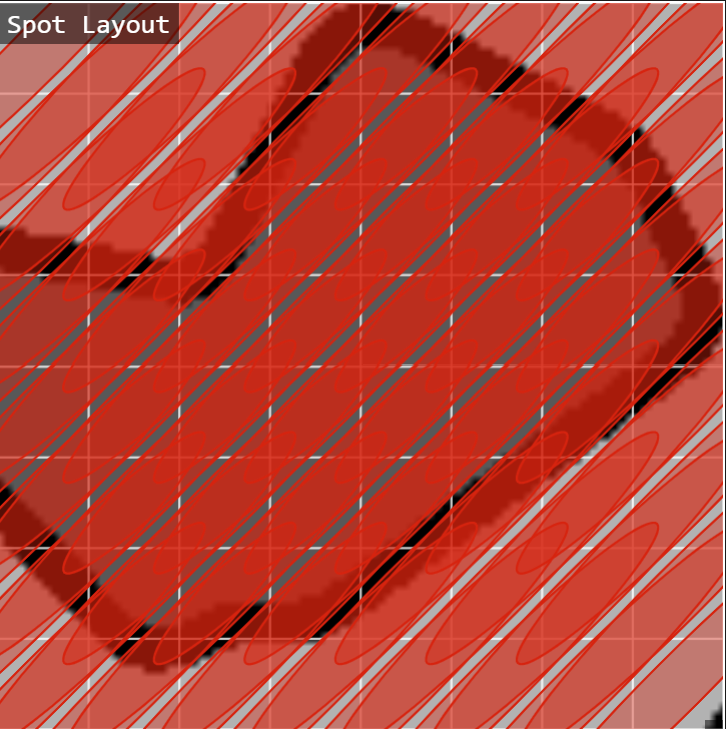
\includegraphics[width=5cm]{t6a.png}
   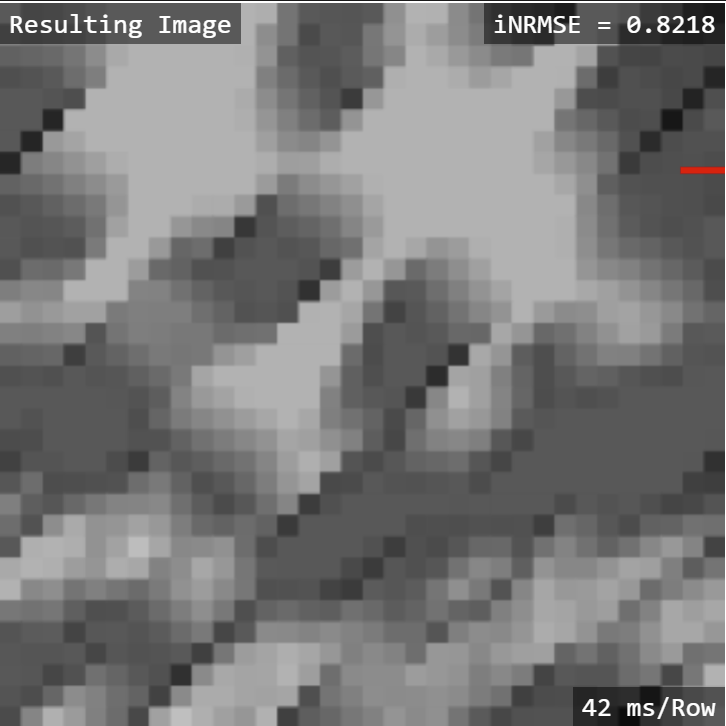
\includegraphics[width=5cm]{t6b.png}
  \caption{The spot layout and resulting image matching the expected test result:
  Spot size of 60 by 500\% at 45 degrees rotation.}
  \label{fig_t6} 
  \end{center}
\end{figure}

\subsubsection{T7: Raster Grid / Pixel Size (R3 and R5)}
The test was passed as shown in figure \ref{fig_t7}.
\begin{figure}[h!]
  \begin{center}
   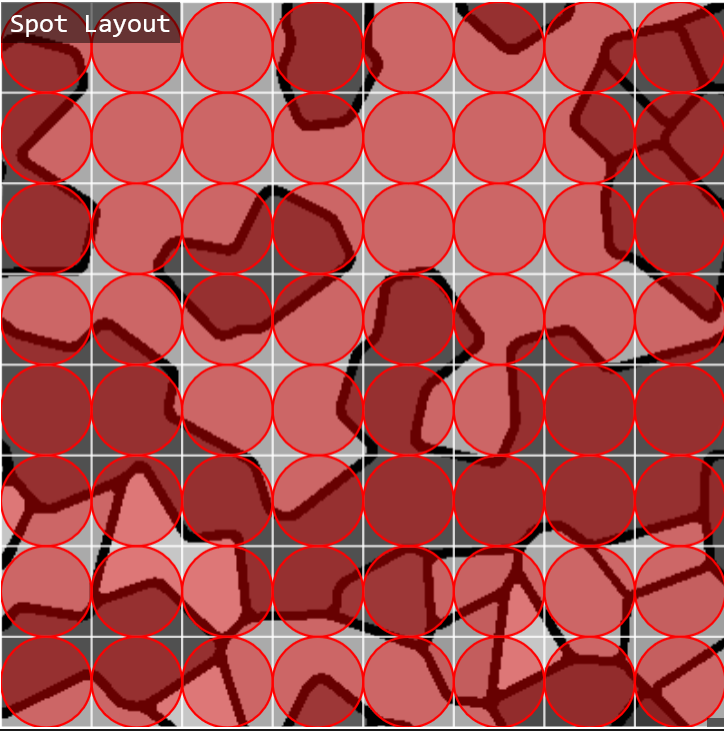
\includegraphics[width=5cm]{t7a.png}
   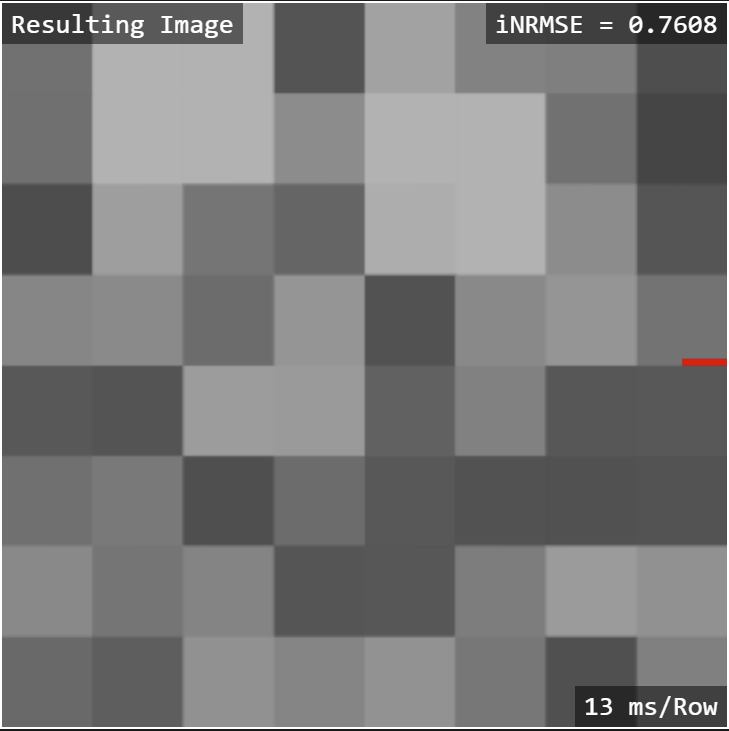
\includegraphics[width=5cm]{t7b.png}
  \caption{The spot layout and resulting image matching the expected test result: an 8 by 8 pixel image.}
  \label{fig_t7} 
  \end{center}
\end{figure}

\subsubsection{T8: Subregion / ROI (R4 and R5)}
The test was passed as shown in figure \ref{fig_t8}.
\begin{figure}[h!]
  \begin{center}
   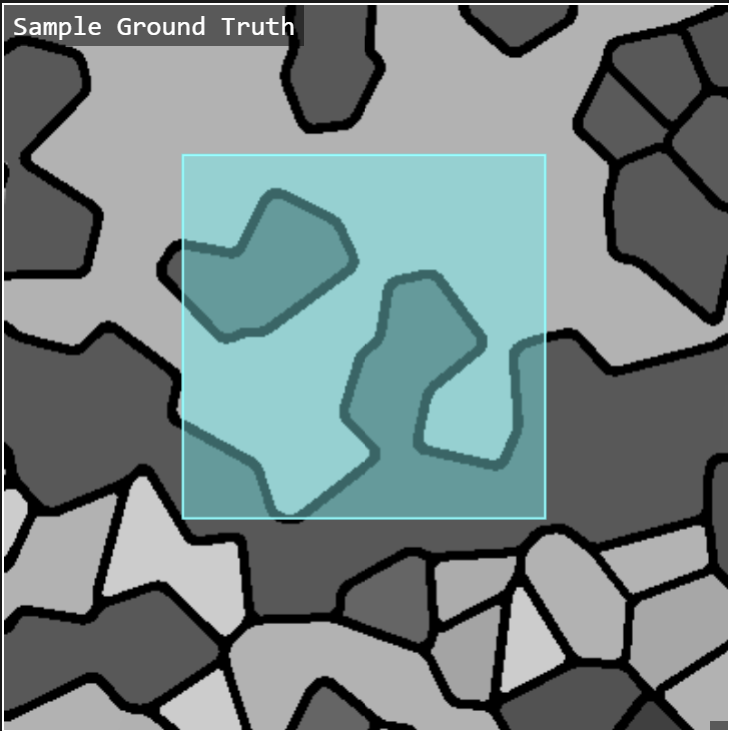
\includegraphics[width=5cm]{t8a.png}
   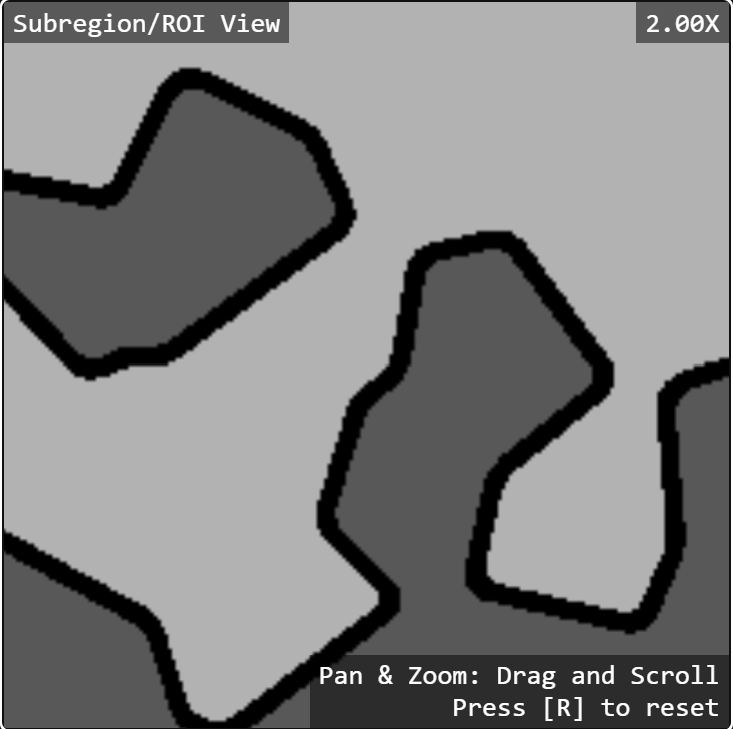
\includegraphics[width=5cm]{t8b.png}
   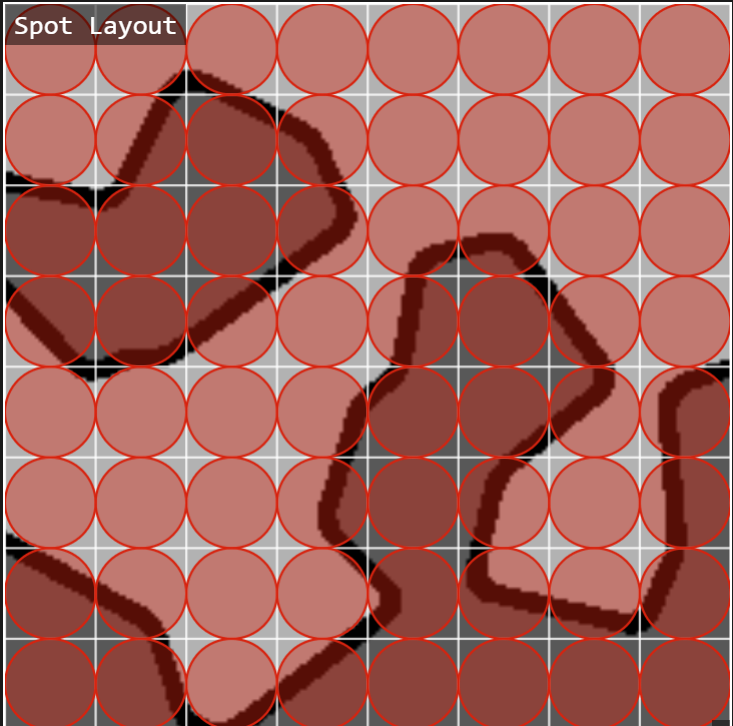
\includegraphics[width=5cm]{t8c.png}
   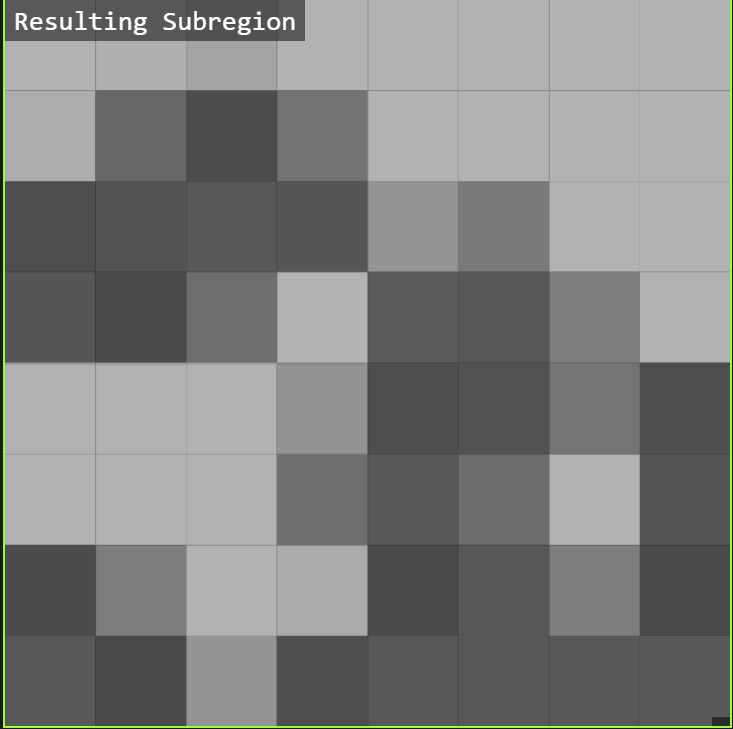
\includegraphics[width=5cm]{t8d.png}
   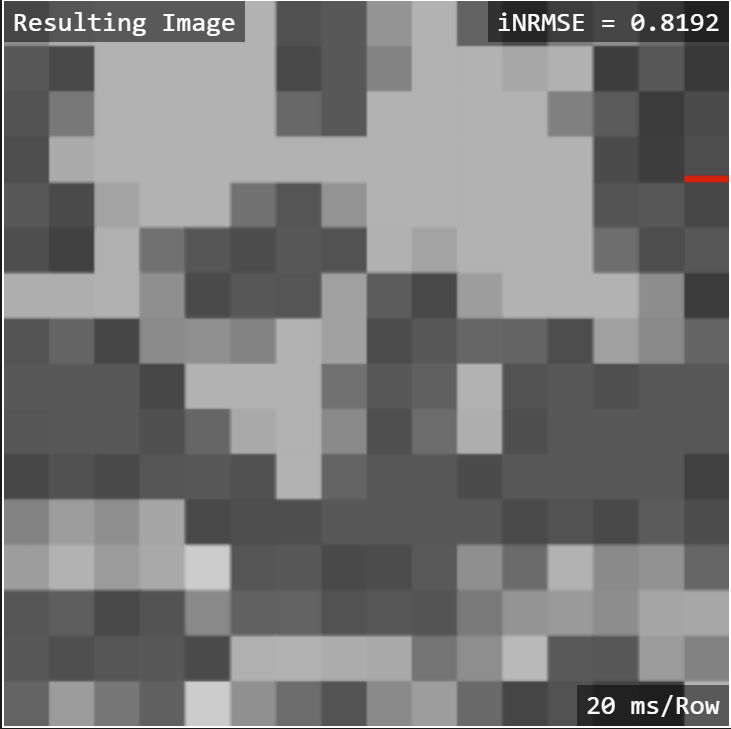
\includegraphics[width=5cm]{t8e.png}
  \caption{The spot layout, subregion, and resulting image matching the expected test result.}
  \label{fig_t8} 
  \end{center}
\end{figure}

\subsubsection{T9: Ground Truth Reproduction (R1, R2, R3, and R6)}
The test was passed as shown in figure \ref{fig_t9}.
\begin{figure}[h!]
  \begin{center}
   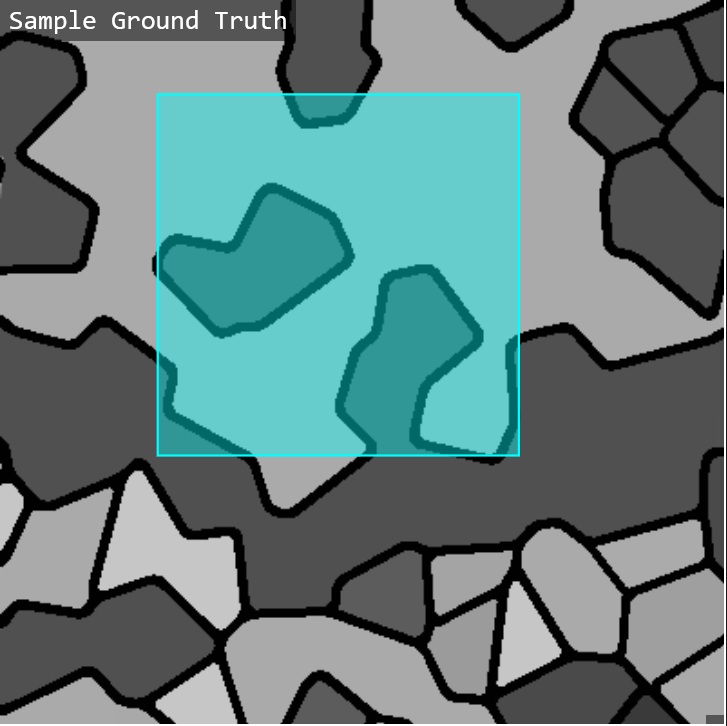
\includegraphics[width=5cm]{t9a.png}
   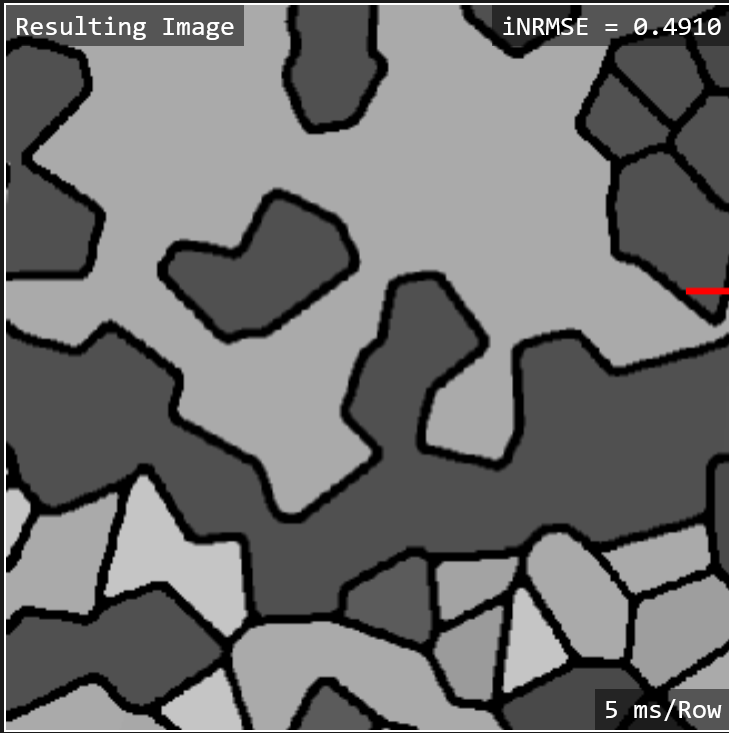
\includegraphics[width=5cm]{t9b.png}
  \caption{The expected test result: the ground image and resulting image are visually identical.}
  \label{fig_t9} 
  \end{center}
\end{figure}


\subsection{Image Quality Metric (R7)}
This section focuses on testing the image quality metric general cases. Naturally,
this is no flawless or foolproof image quality metric. Over 20 different image metrics have been
reviewed and compared by Jagalingam and Hegde in a 2015 paper,
each with their different strengths and weaknesses \cite{JAGALINGAM2015133}.

\subsubsection{T10: High metric value (approximate to exact-sampling)}
The test was passed as shown in figure \ref{fig_t10}.
\begin{figure}[h!]
  \begin{center}
   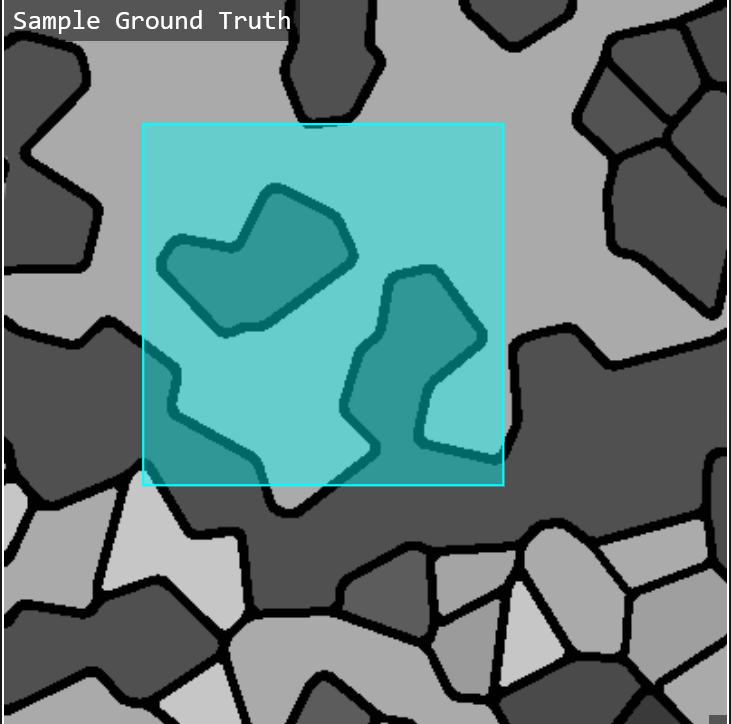
\includegraphics[width=4cm]{t10a.png}
   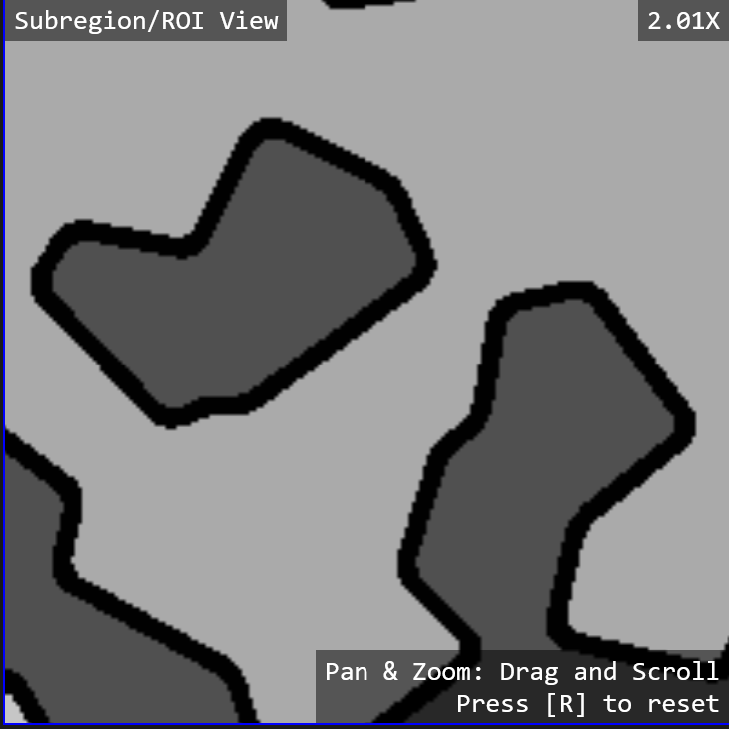
\includegraphics[width=4cm]{t10b.png}
   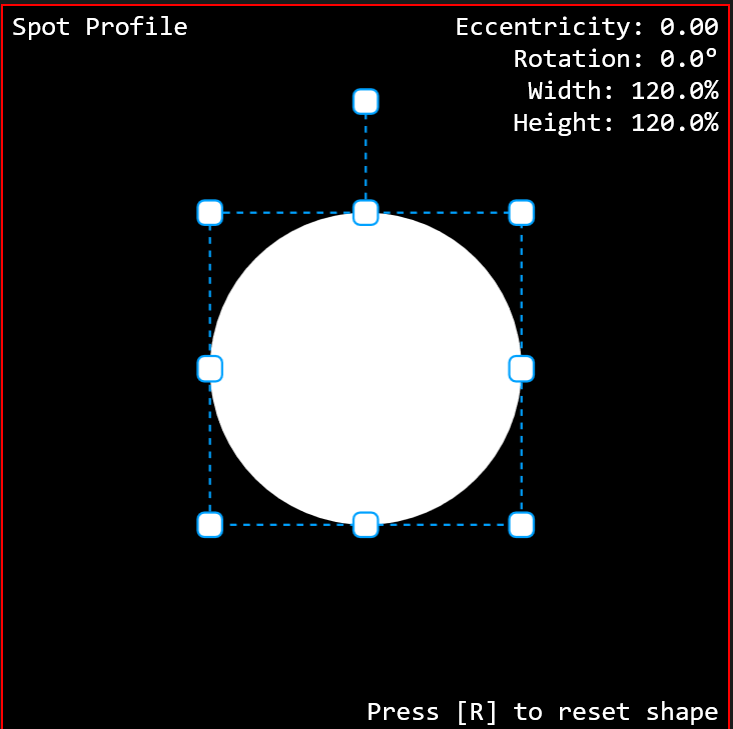
\includegraphics[width=4cm]{t10c.png}
   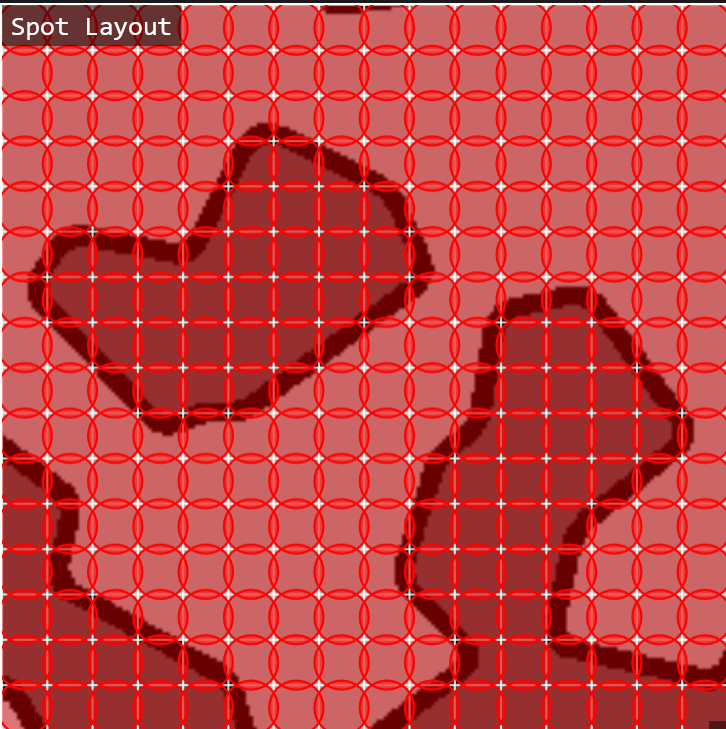
\includegraphics[width=4cm]{t10d.png}
   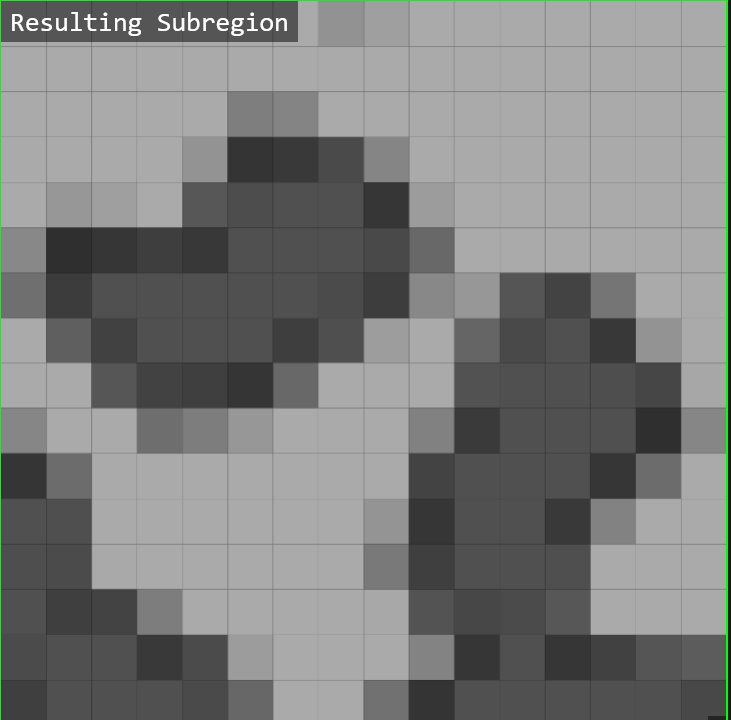
\includegraphics[width=4cm]{t10e.png}
   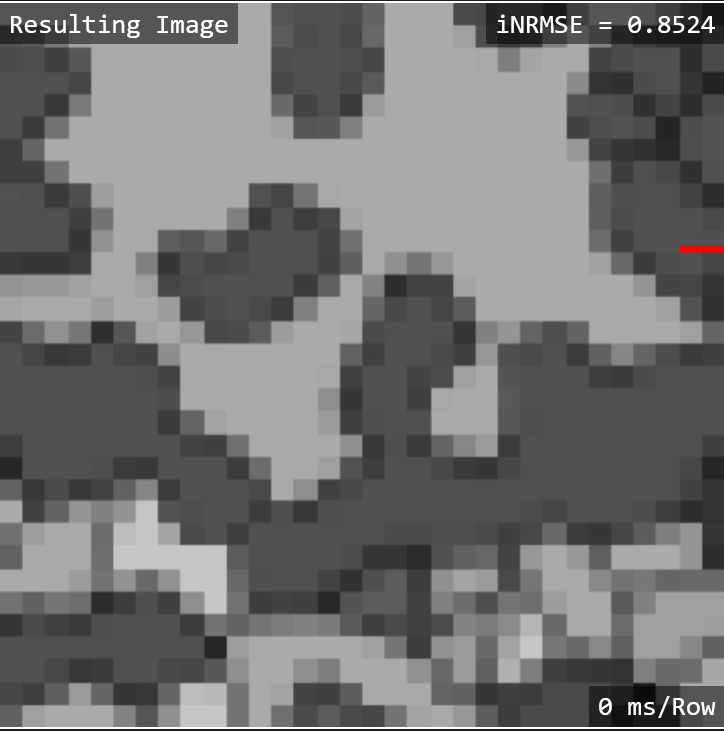
\includegraphics[width=4cm]{t10f.png}
  \caption{The spot layout, spot profile, subregion, and resulting image with a score equal or greater to
  the expected test result of a ``0.8501'' minimum.}
  \label{fig_t10} 
  \end{center}
\end{figure}

\subsubsection{T11: Low metric value (under-sampling)}
The test was passed as shown in figure \ref{fig_t11}.
\begin{figure}[h!]
  \begin{center}
   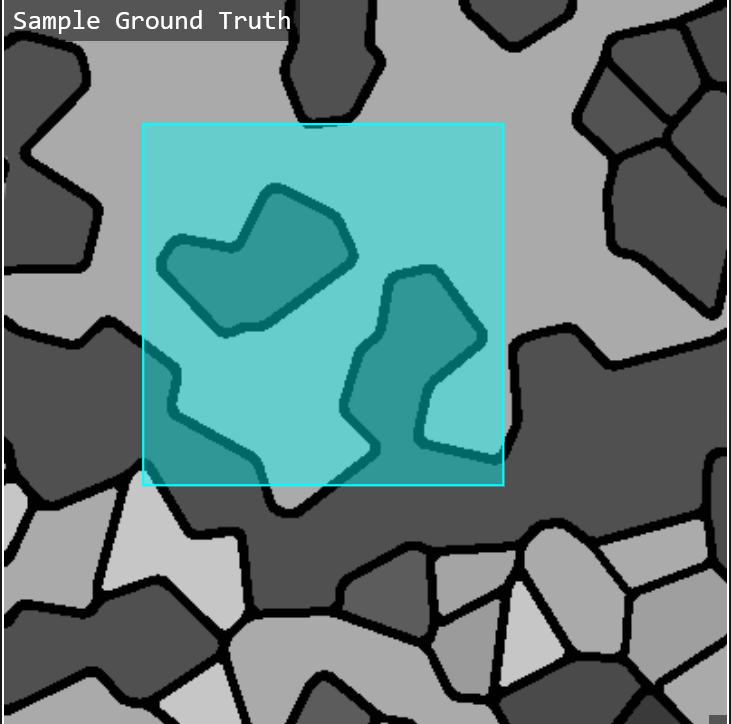
\includegraphics[width=4cm]{t10a.png}
   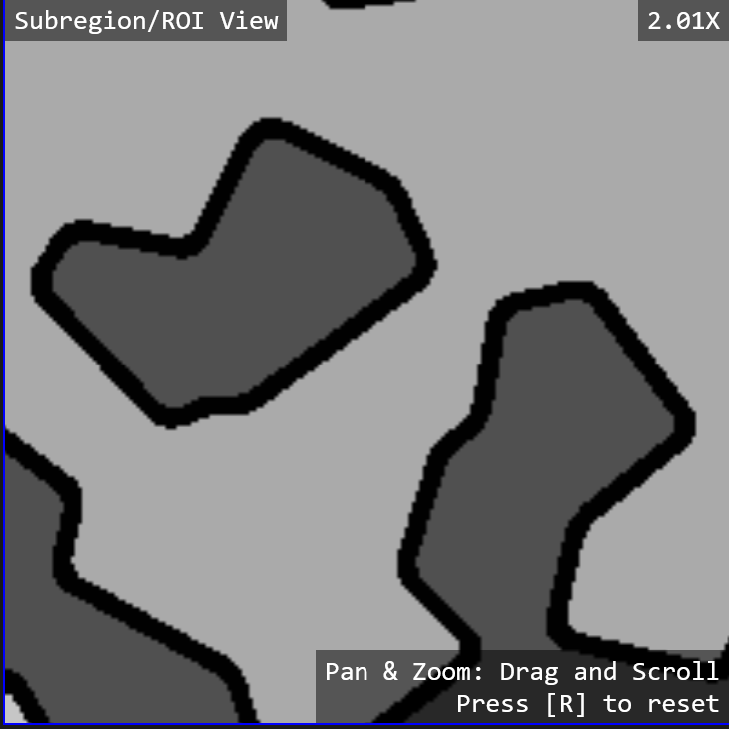
\includegraphics[width=4cm]{t10b.png}
   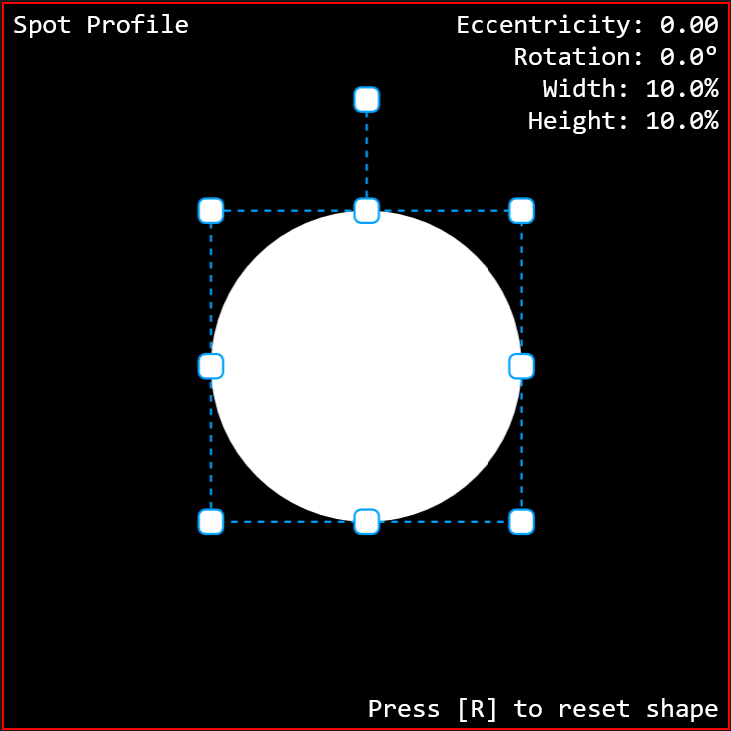
\includegraphics[width=4cm]{t11c.png}
   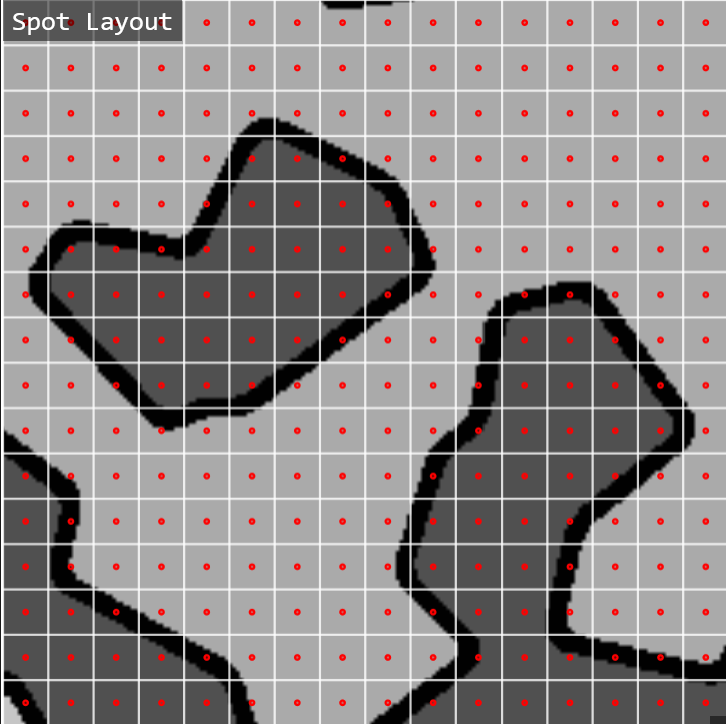
\includegraphics[width=4cm]{t11d.png}
   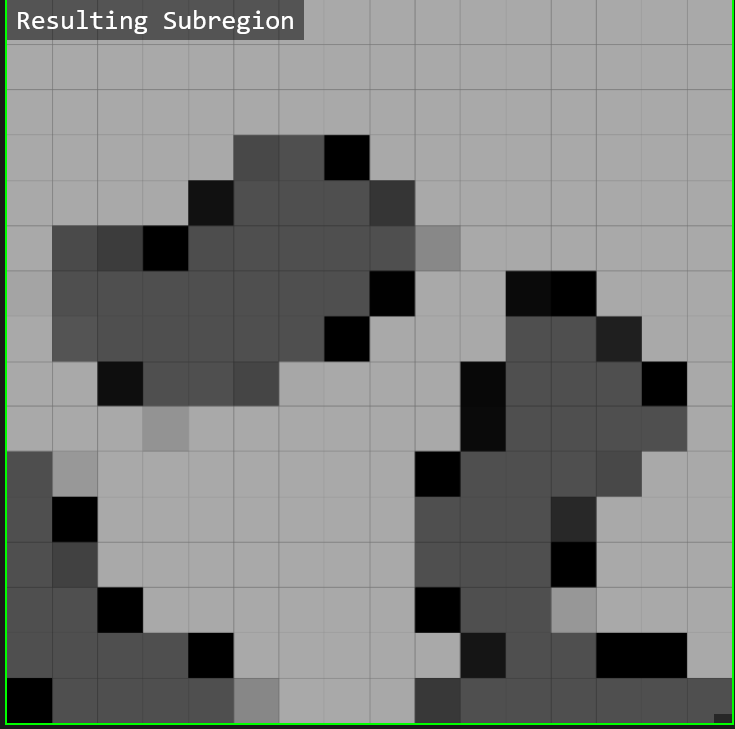
\includegraphics[width=4cm]{t11e.png}
   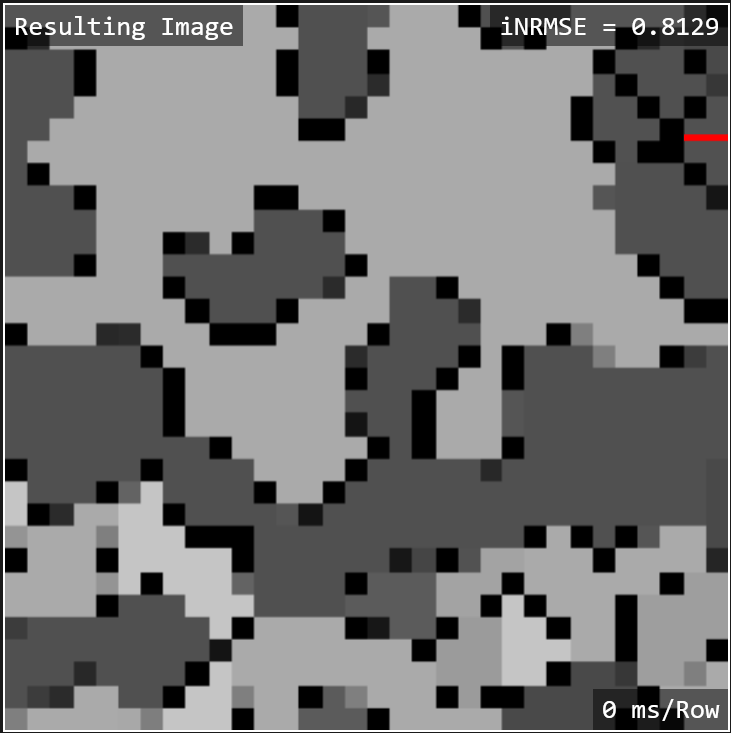
\includegraphics[width=4cm]{t11f.png}
  \caption{The spot layout, spot profile, subregion, and resulting image with a score less or equal to
  the expected test result of a ``0.8501'' maximum.}
  \label{fig_t11} 
  \end{center}
\end{figure}

\subsubsection{T12: Low metric value (over-sampling)}
The test was passed as shown in figure \ref{fig_t12}.
\begin{figure}[h!]
  \begin{center}
   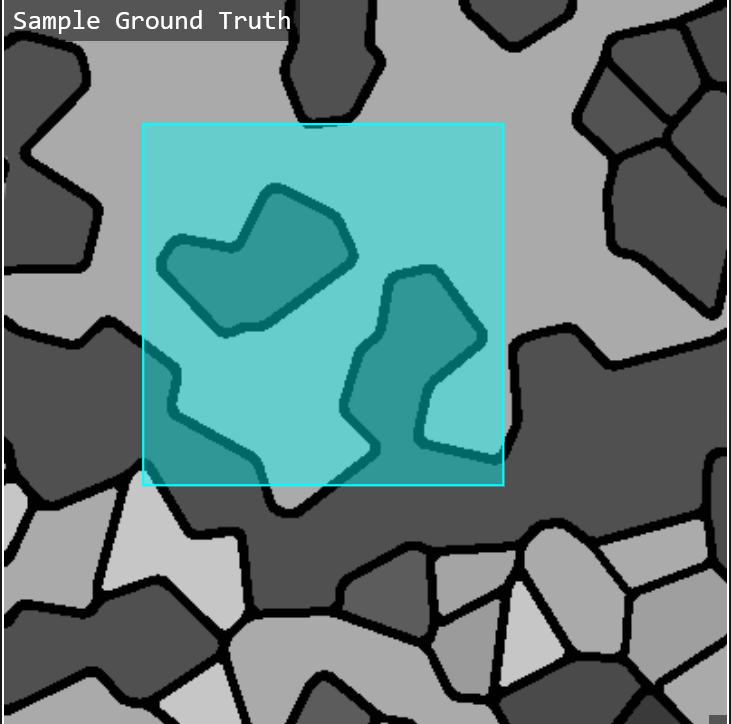
\includegraphics[width=4cm]{t10a.png}
   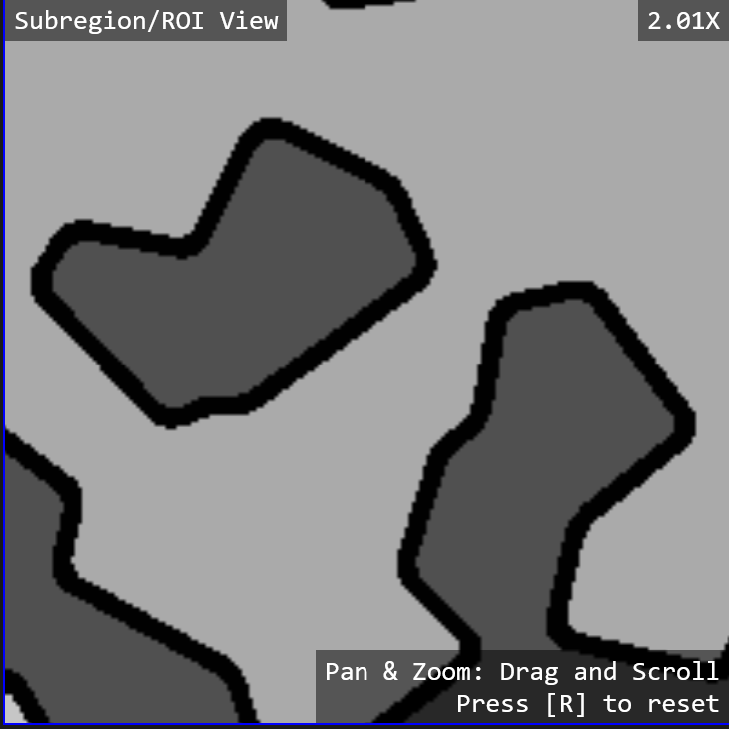
\includegraphics[width=4cm]{t10b.png}
   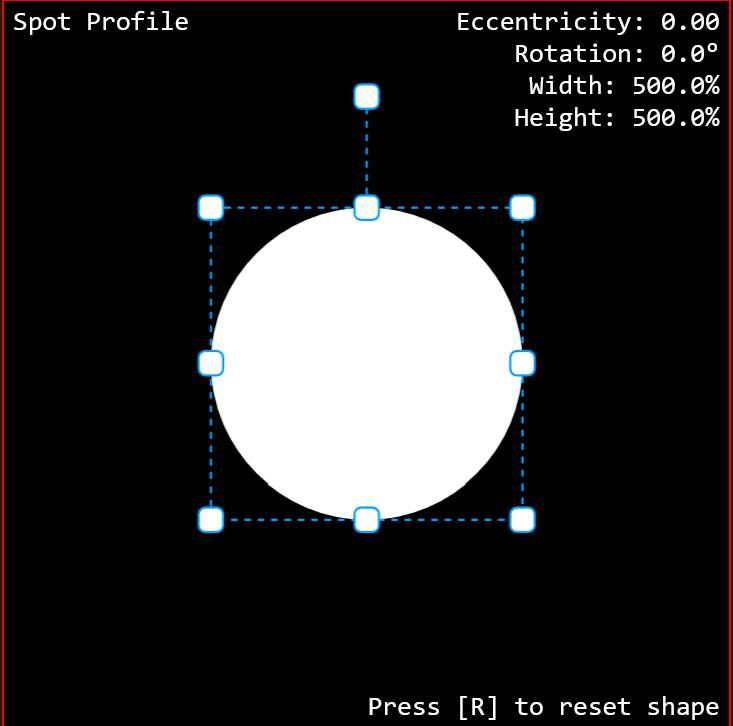
\includegraphics[width=4cm]{t12c.png}
   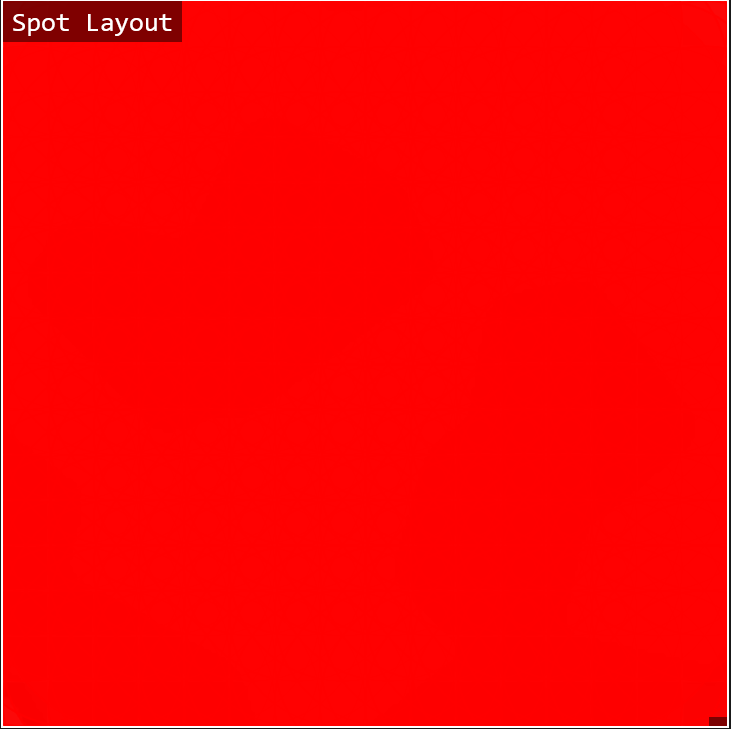
\includegraphics[width=4cm]{t12d.png}
   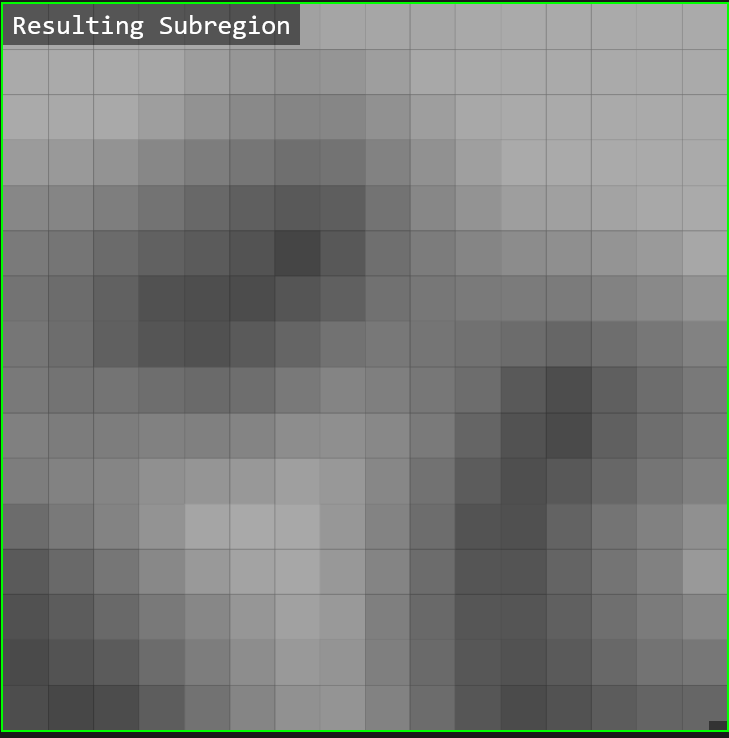
\includegraphics[width=4cm]{t12e.png}
   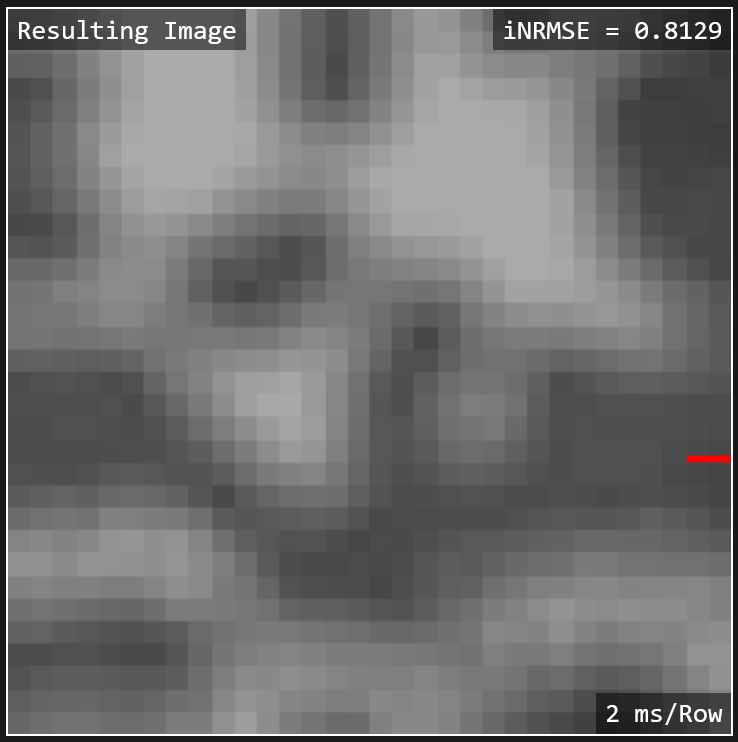
\includegraphics[width=4cm]{t12f.png}
  \caption{The spot layout, spot profile, subregion, and resulting image with a score less or equal to
  the expected test result of a ``0.8501'' maximum.}
  \label{fig_t12} 
  \end{center}
\end{figure}

\subsubsection{T13: Control metric value} \label{T13}
The test was passed as shown in figure \ref{fig_t12}.
\begin{figure}[h!]
  \begin{center}
   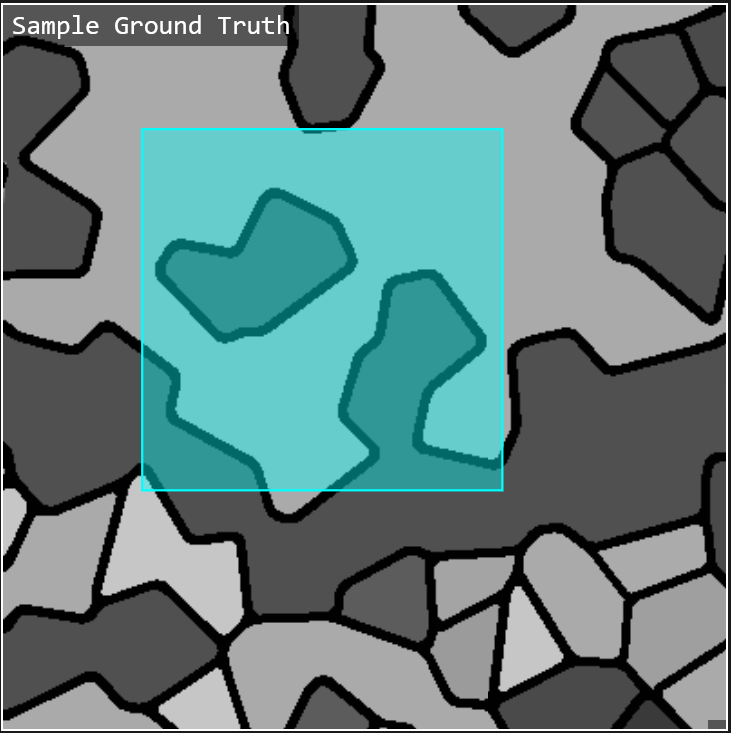
\includegraphics[width=5cm]{t13a.png}
   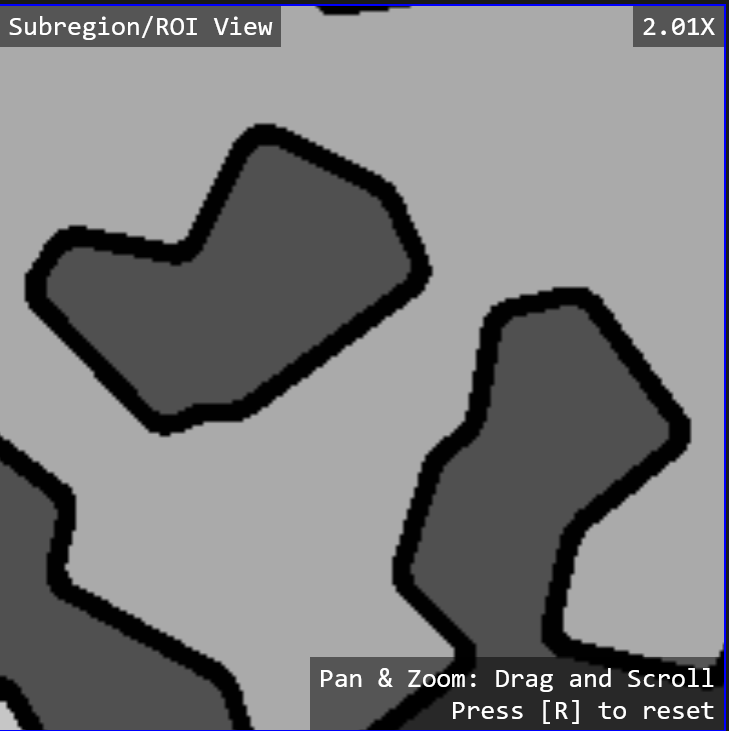
\includegraphics[width=5cm]{t13b.png}
   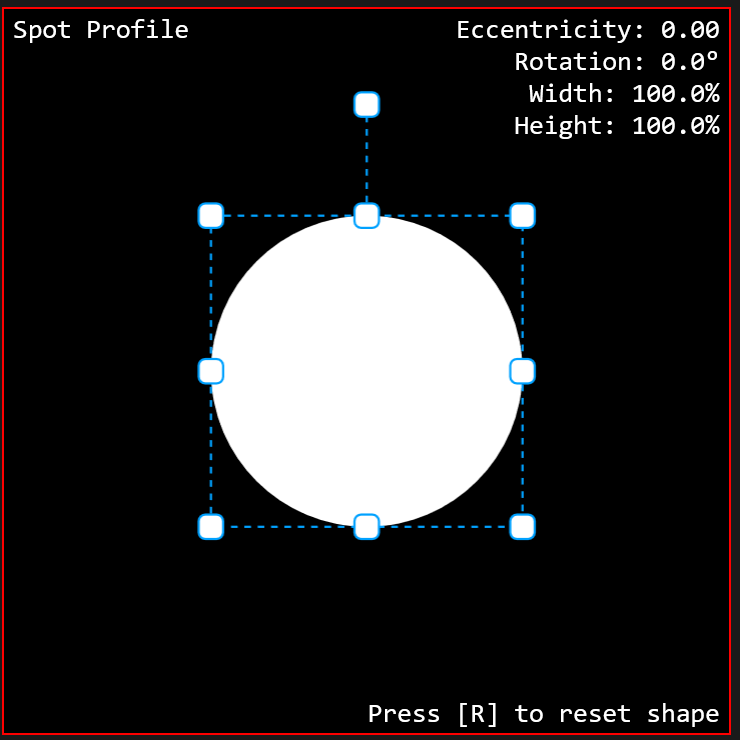
\includegraphics[width=5cm]{t13c.png}
   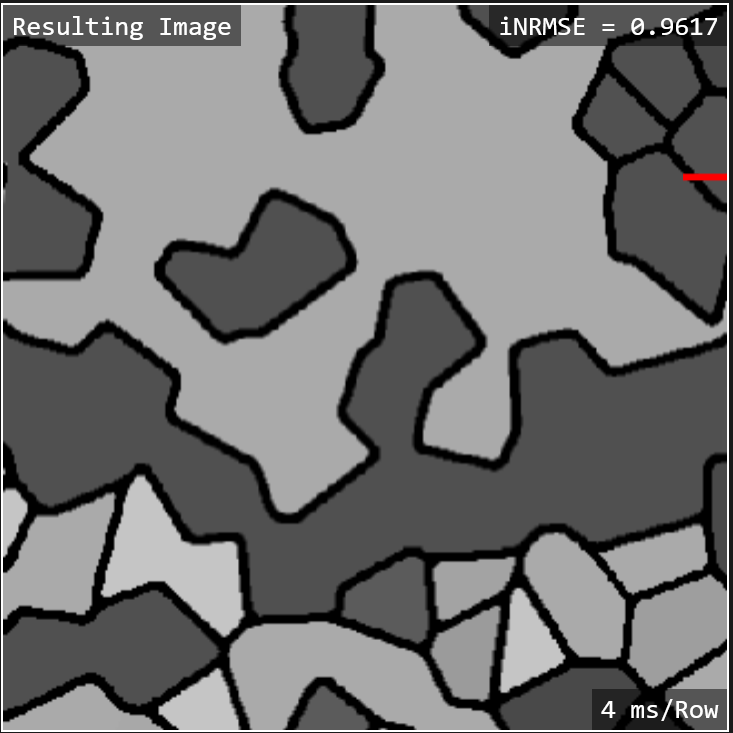
\includegraphics[width=5cm]{t13d.png}
  \caption{The spot layout, spot profile, subregion, and resulting image with a score greater or equal to
  the expected test result of a ``0.9500'' minimum.}
  \label{fig_t12} 
  \end{center}
\end{figure}




\newpage
\clearpage

\section{Nonfunctional Requirements Evaluation}
This section focuses on the testing results verifying whether the nonfunctional requirements
(as defined in the SRS \cite{SRS}) are met. Emphasis is put on the \textit{usability} and
by extension \textit{portability}: The software should be easy to set up and use without
having to worry about any technicalities that could otherwise hinder or completely
prohibit non "tech-savvy" individuals from using the software.

\subsection{Usability}
\subsubsection{T14: Usability Survey (NFR2)}
The usability survey was not completed. The software was casually reviewed in verbal discussion
with the expert consultants (as listed in the VnV Plan \cite{VnV_plan})
throughout the development of the software. Suggested features and minor issues has been
implemented into the software such as: the ability to set a spot size by numeric input,
draw the resulting row-by-row for responsiveness, and a display for spot shape eccentricity.

\subsection{Accuracy}
\subsubsection{T15: Image Metric Survey (NFR1)}
The image quality survey was not executed, but shall be some time in the future.

\subsection{Maintainability}
\subsubsection{T16: Static code analysis (NFR3)}
...
\subsubsection{T17: Code Review (NFR3)}
...

\subsection{Portability}
\subsubsection{T18: Various Platforms and Environments (NFR4)}
...
	
\section{Comparison to Existing Implementation}	

This section will not be appropriate for every project.

\section{Unit Testing}

\section{Changes Due to Testing}
\begin{enumerate}
  \item The passing value for T13 (see \ref{T13}) had to be changed from ``0.9800'' to `0.9500' since the
    resulting images look identical. The resulting value of `0.9617' seemed satisfactory and the original
    expected test value was perhaps too constrained.
\end{enumerate}


\section{Automated Testing}
		
\section{Trace to Requirements}
		
\section{Trace to Modules}		

\section{Code Coverage Metrics}


\bibliographystyle{plainnat}
\bibliography{../../refs/References,../../refs/cas741,../../refs/algorithms}


\newpage{}
\section*{Appendix --- Reflection}

The information in this section will be used to evaluate the team members on the
graduate attribute of Lifelong Learning.  Please answer the following questions:

\begin{enumerate}
  \item 
  \item 
\end{enumerate}

\end{document}